\chapter{�bung 27.10.2012}
Ein Protokoll der Schicht 1 ist realisiert auf Basis des NZR Protokolls mit 4B/5B Blockkodierung mit einer �bertragungsfrequenz von max. 10 MHz.\\
Beantworten Sie folgende Fragen und begr�nden Sie Ihre Antworten.\\


\renewcommand{\labelenumi}{\alph{enumi})}
\begin{enumerate}
%
\item Handelt es sich um eine Basisband oder eine Breitband �bertragung?

Es handelt sich um ein Basisband.\\
Begr�ndung: Das Signal wird mittels NZR 4B/5B ummoduliert �bertragen.\\
Es gibt keine Tr�gerfrequenz (=Breitband).

\small{\textbf{Anmerkung Basisband/Breitband} \\
Bei der �bertragungstechnologie unterscheidet man zwischen Basisband und Breitband. Bei Basisband�bertragungen wird das Signal unmoduliert direkt auf das �bertragungsmedium gelegt. Es kann nur ein Signal w�hrend einer Zeit �bertragen werden. Eine Koexistenz von Signalen ist ohne gegenseitige Beeinflussung nicht m�glich. Die �bertragungsraten liegen zurzeit bei etwa 10 Gbit/s. Das bekannteste Basisbandnetz ist das Ethernet, das in IEEE 802.3 und ISO 8802/3 standardisiert ist.\\
Im Gegensatz zum Basisband werden die Signale bei Breitband�bertragungen auf eine Tr�gerfrequenz moduliert und belegen in einer Vielzahl zur Verf�gung stehender Frequenzb�nder ein Frequenzband. Die Frequenzb�nder k�nnen gleichzeitig f�r die �bertragung mehrerer Daten-, Video- und Audio-Kan�le benutzt werden, ohne sich gegenseitig zu beeinflussen.\\
\textit{Quelle:\\http://www.itwissen.info/definition/lexikon/Uebertragungstechnologie-transmission-technology.html}}\\ \normalsize

\item Welche Bitrate wird erzielt?

Bei $10$ MHz werden pro Sekunde $10 \cdot 10^6$ Bits �bertragen.\\
Es k�nnen jedoch nur 4 von 5 Bits effektiv benutzt werden.\\
Somit ist die Nutzbitrate = $4/5 \cdot Bitrate =  $\textbf{8 Mbit/sec}\\

\item Welche Kabel der EIA/TIA Kategorisierung sind geeignet?

F�r diese Anwendung w�rde ein Cat-3-Kabel gen�gen.

\small{Cat-3-Kabel sind nicht abgeschirmte Twisted-Pair-Kabel, die auf maximale Betriebsfrequenzen von 16 MHz ausgelegt sind und f�r �bertragungskapazit�ten von bis zu 16 Mbit/s verwendet werden.}\normalsize

\item Vergleichen Sie das Protokoll hinsichtlich Clockrecovery und dem Verh�ltnis\\ �bertagungsfrequenz/Bitrate mit einem Protokoll welches Manchester Codierung �ber 10 MHz realisiert.

Manchester: es werden immer 2 Bit pro Nutzbit �bertragen.\\
$=>$ Nutz-Bitrate = $0.5 \cdot 10 Mbit/sec = 5 Mbit /sec$
 
 \begin{tabular}[t]{|l|c|c|c|} \hline
 \rowcolor{darkgrey} & &  & \\
\rowcolor{darkgrey}
\multirow{-2}{1.7cm}{\textbf{Variante}} &
\multirow{-2}{2.25cm}{\textbf{Clock Recovery}}&
\multirow{-2}{2.5cm}{\textbf{Nutz-Bitrate}}  &
\multirow{-2}{5cm}{\textbf{�bertragungsfrequenz / Nutz-Bitrate}} \\
NRZ & nicht gegeben  & $8 Mbit/sec$ & 1.25  \\ \hline 
Manchester & gegeben  & $5 Mbit/sec$ & 2 \\  \hline 
\end{tabular}\\

\item Welche maximale L�nge ergibt sich f�r u.g. Glasfaserkabel (Varianten A-D) unter Verwendung des unter 1. beschrieben Protokolls bei 850nm und 1300 nm Wellenl�nge?

Info: mit NZR und 4B/5B



\small{
\begin{tabular}[t]{|l|c|c|c|c|} \hline
\rowcolor{darkgrey} & &  & & \\
\rowcolor{darkgrey}
\multirow{-2}{1.7cm}{\textbf{Variante}} &
\multirow{-2}{2.25cm}{\textbf{MHz $\cdot$ km bei 850nm}}&
\multirow{-2}{2.5cm}{\textbf{max. L�nge bei 850nm}}  &
\multirow{-2}{2.25cm}{\textbf{MHz $\cdot$ km bei 1300nm}} &
\multirow{-2}{2.5cm}{\textbf{max. L�nge bei 1300nm}} \\
A & 400  & $400/10MHz = 40 km$ & 1200 & $1200/10MHz = 120 km$ \\ \hline 
B & 400  & $400/10MHz = 40 km$ & 800 & $800/10MHz = 80 km$\\  \hline 
C & 400  & $400/10MHz = 40 km$ & 400 & $400/10MHz = 40 km$\\  \hline 
D & 200  & $200/10MHz = 20 km$ & 400 & $400/10MHz = 40 km$\\  \hline 
  \end{tabular}
}
\item Welche der o.g. Kabelvarianten (A-D) erreichen diese maximale L�nge bei 850nm und 1300nm Wellenl�nge?

????????????????\\
\end{enumerate}
\newpage
\section{Anhang}

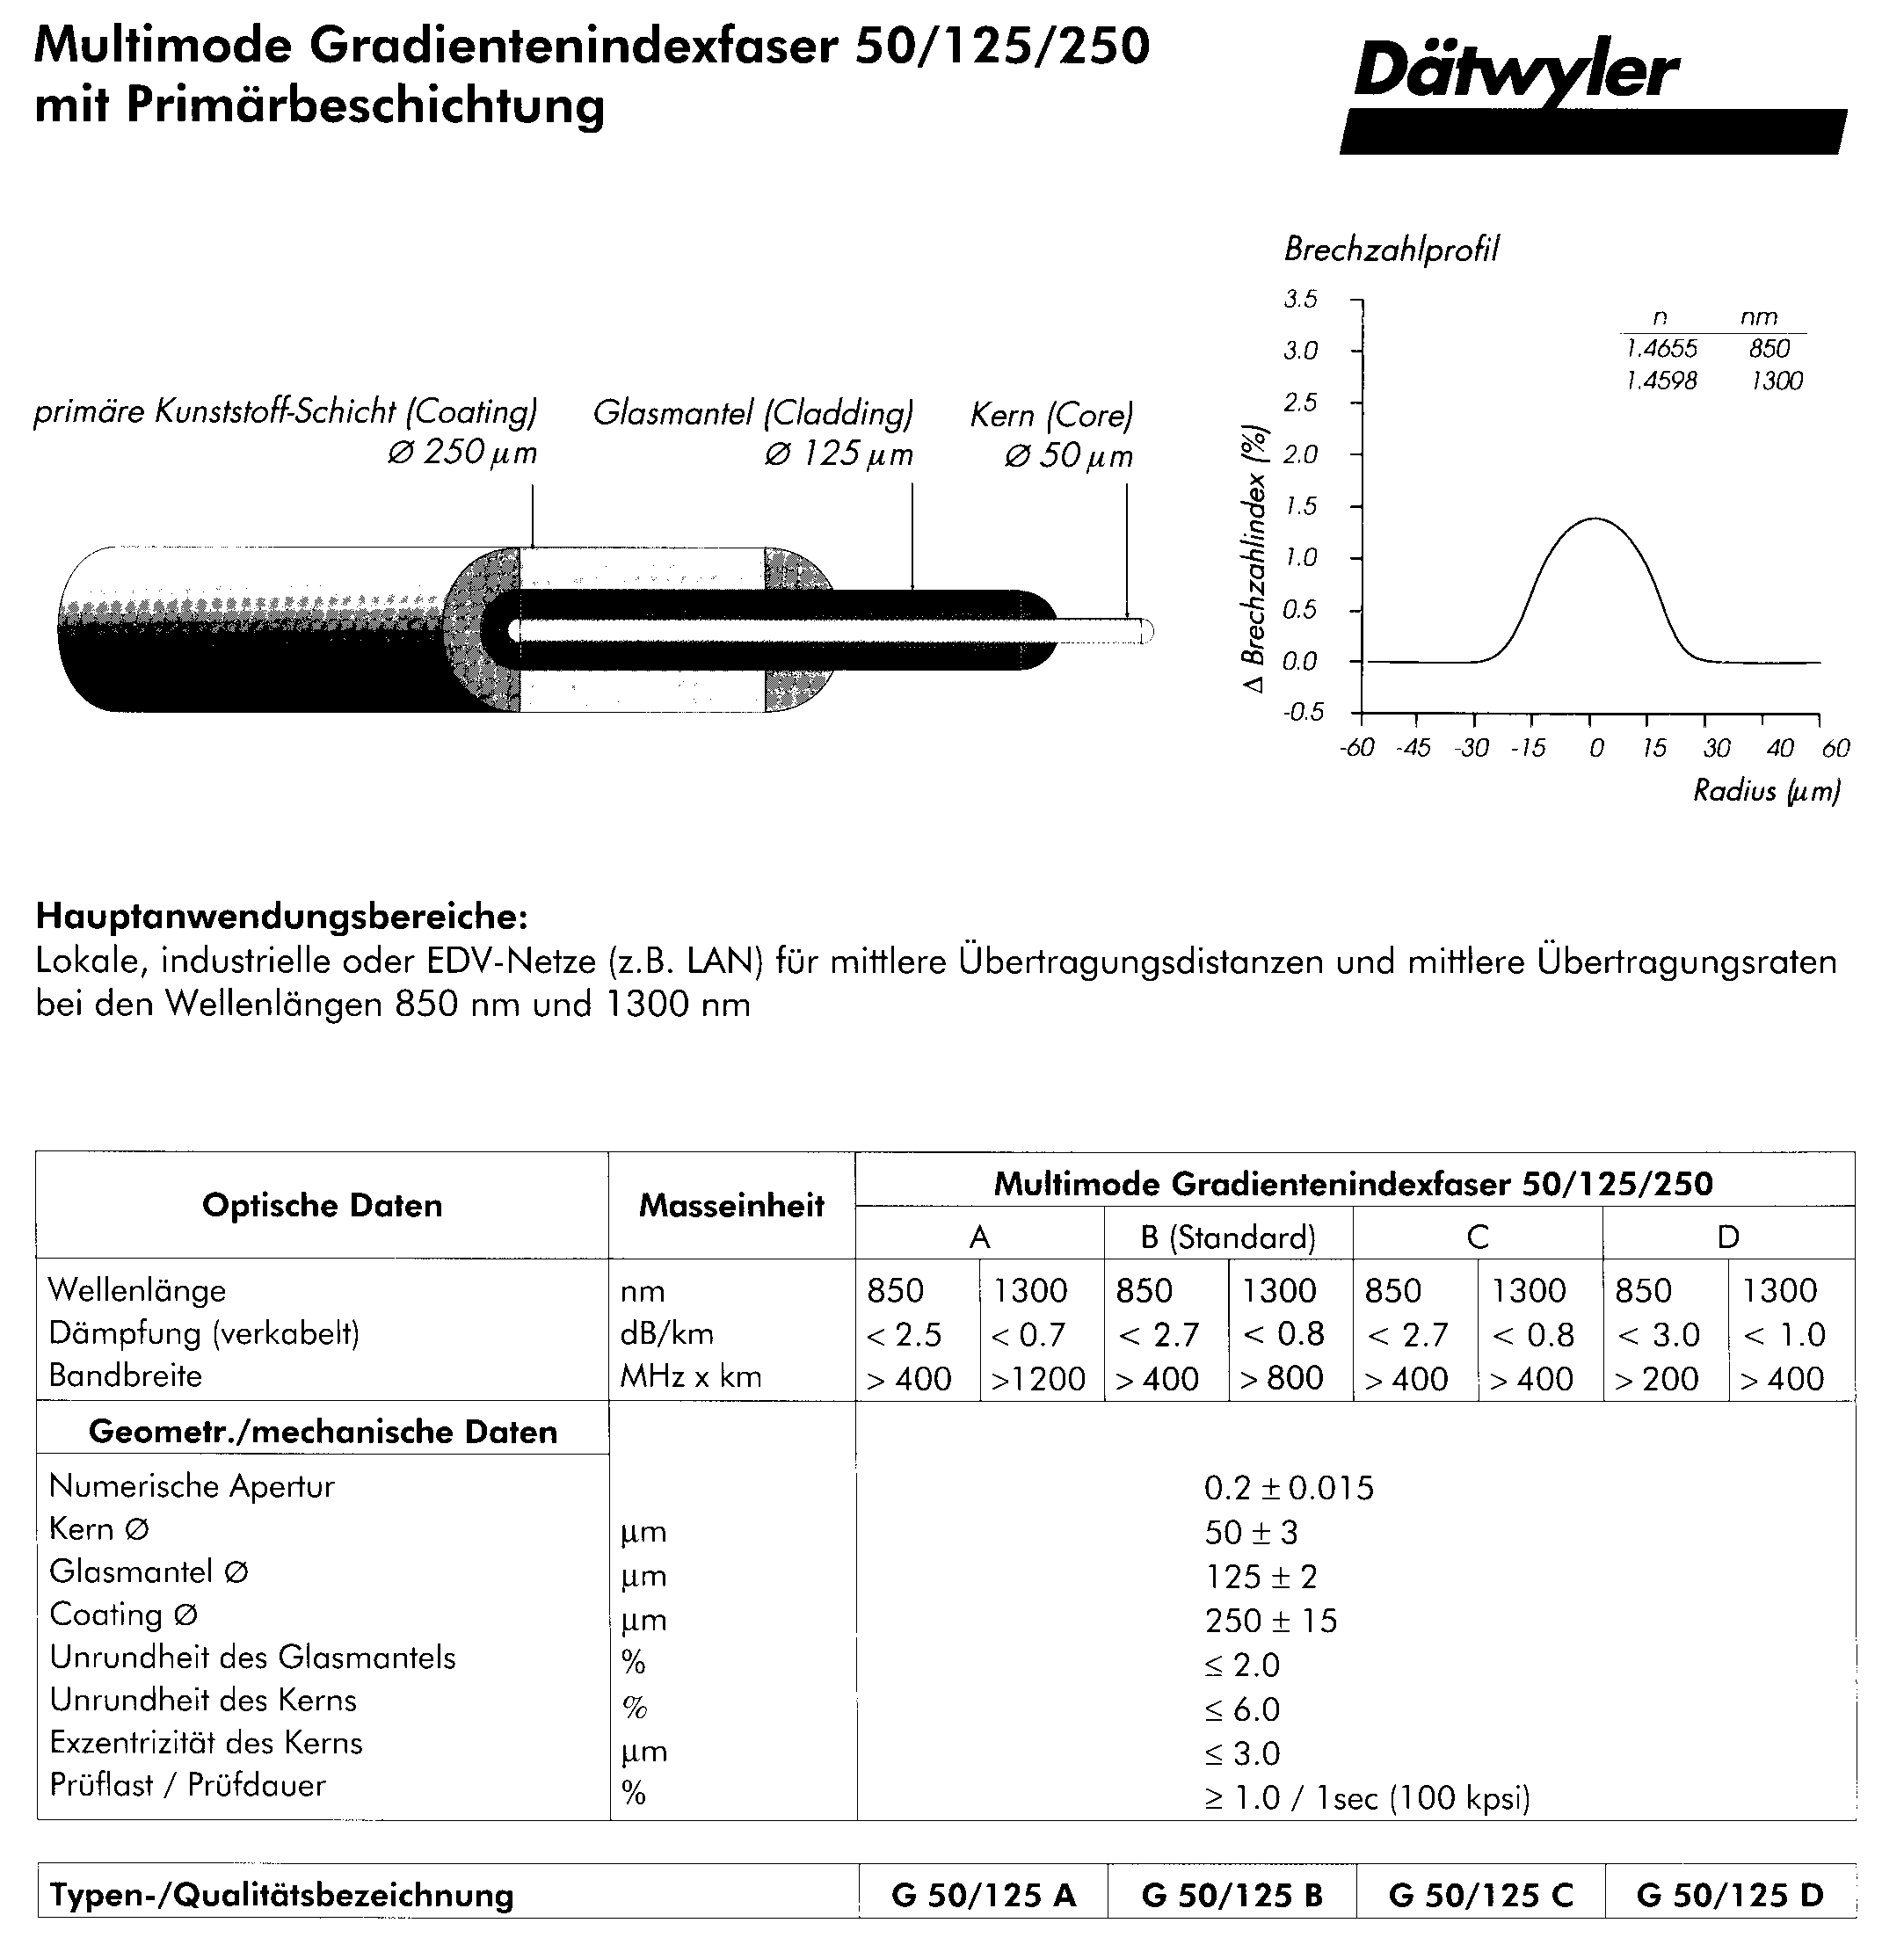
\includegraphics[width=18cm]{Library/Uebung_27-10-2012/LWL-Kabel.png}

